% !TeX spellcheck = en_UK

\section{3C295 and the Extended Groth Strip}\label{section.3c295+EGS}
\pg
In this section, we describe the work done as part of this PhD on calibrating and imaging interferometric data on the Boötes field, an extragalactic field with rich multi-wavelength coverage. This work can be described in two parts: first, we created a high-resolution, multi-wavelength model of a bright, diffuse source near the field, 3C295. Only with this model could work on the Extended Groth Strip begin: without the model, the noise in the image would be dominated by artefacts rather than thermal noise, and so sensitivity would not increase with additional data. 

\pg
This section is thus logically split into two separate parts. First, we discuss obtaining a high-resolution, multi-wavelength model for 3C295. Then, we show the work done investigating whether direction-dependent effects were strong enough to require a multi-facet calibration of the Extended Groth Strip.


\subsection{Modelling a calibrator source: 3C295}\label{section.3c295}

\pg
Let us begin by describing the method used to acquire a high-quality, high-resolution multi-wavelength model of 3C295. 

\subsubsection{Initial Model}
\pg
The initial model was acquired from the NASA/IPAC Extragalactic Database\footnote{\hyperref[here]{https://ned.ipac.caltech.edu/}}. PyBDSM \citep{2015ascl.soft02007M} was used to extract a two-point model from a $0.2''$ VLA image \citep[see][]{1991AJ....101.1623P}. The image is shown in Fig. \ref{fig.vla.3c295}.

\begin{figure}[h!]\label{fig.vla.3c295}
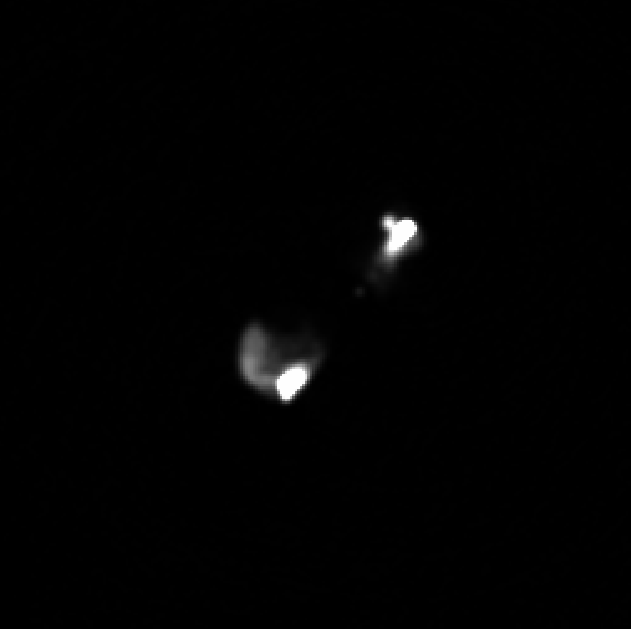
\includegraphics[width=\linewidth]{images/3c295-vla}
\caption{VLA observation of 3C295. Pixel size is $0.2''$.}
\end{figure}




\newpage

plan:
 - acquire basic model (find examples on NED, show which, show how extraction of two peaks only was performed)
 - describe dataset: time, frequency, subbands, channels etc
 - self-calibrate on a single subband, sb093, as test
   -> describe strategy:
     . find international station sols first!
     . means flagging core stations - this breaks horrendously...
     . debate w/ leah
   -> describe improvement between self-cal rounds:
     . noise decreases in visibilities
     . artefacts (+ ghosts, cite trienko) decrease in image-plane
 - self-calibrate sets of subbands with wide-BW deconvolution
 - ???
 - success: MWL model into low-freqs






\newpage
\subsection{The Boötes field}\label{subsection.EGS}

\pg
The Extended Groth Strip (henceforth, EGS) is one of the so-called ``famous extragalactic fields". has been long observed as part of the All-Wavelength Extended Groth Strip International Survey collaboration (\citepads{2007ApJ...660L...1D}), which later became part of the CANDELS collaboration (\citepads{2011ApJS..197...35G}). The field is centred at $\alpha=14^h17^m,\delta=+52\deg 30'$, placing it between the tail of Ursa Major and Draco. The $\lambda$-coverage is summarised in \cref{bootes-coverage-table}, and the associated pointings given in \cref{bootes-coverage-image}

%\newpage

\begin{table}[h!]
\centering
\caption{Multi-wavelength coverage of the Boötes field}
\label{bootes-coverage-table}
\begin{tabular}{|ccccc|} \hline
Catalog                    & $\lambda$,$\nu$,band           & Sensitivity              & Resolution               & Source                            \\\hline\hline
XBootes                    & 0.5-0.7 keV                    & $4(8).10^{-15}$ ergs cm$^{-2}\text{s}^{-1}$ & 0.492''                & \citepads{2005ApJS..161....1M}    \\\hline
\multirow{6}{*}{NOAO-Deep} & B$_\text{W}$                   & 26.6 mag                 & \multirow{6}{*}{1''\footnote{Seeing-limited. Value given at: \url{https://www.noao.edu/noao/noaodeep/DR3/optimagepropsdr3.html}}}                                              &\multirow{6}{*}{\citepads{1999ASPC..191..111J}}\\
                           & R                              & 25.8 mag                 &                          &                                   \\
                           & I                              & 25.5 mag                 &                          &                                   \\
                           & J                              & 20.2 mag                 &                          &                                   \\
                           & H                              & 19.6 mag                 &                          &                                   \\
                           & K                              & 19.5 mag                 &                          &                                   \\\hline
\multirow{4}{*}{WISE}      & $22\mu$m                       & 5.9 mJy                  & \multirow{4}{*}{1.375''\footnote{Value taken from the \hyperlink{http://wise2.ipac.caltech.edu/docs/release/allsky/expsup/sec1_2.html}{Executive Summary of WISE All-Sky Release Data Products}, under section I.2.a. Image Atlas}} &\multirow{4}{*}{\citepads{2012wise.rept....1C}}              \\
                           & $12\mu$m                       & 0.73 mJy                 &                          &                                   \\
                           & $4.6\mu$m                      & 0.1 mJy                  &                          &                                   \\
                           & $3.4\mu$m                      & 0.048 mJy                &                          &                                   \\\hline
WSRT                       & 1.4 GHz                        & 0.028 mJy                & 13''$\times$27''         & \citepads{2002AJ....123.1784D}    \\
VLA                        & 324.5 MHz                      & 0.5 mJy                  & 6''                      & \citepads{2015MNRAS.450.1477C}    \\
GMRT                       & 153 MHz                        & 5 mJy                    & 26''$\times$22''         & \citepads{2011AnA...535A..38I}    \\
LOFAR-HBA                  & 144 MHz                        & TBA                      & 1.5''                    &   TBA                             \\\hline
\multirow{3}{*}{LOFAR-LBA} & 62 MHz                         & 25 mJy                   & 4''                      & \multirow{3}{*}{\citepads{2014ApJ...793...82V}}    \\
                           & 46 MHz                         & 40 mJy                   & 5''                      &                                   \\
                           & 34 MHz                         & 60 mJy                   & 7''                      &                                   \\\hline
\end{tabular}
\end{table}

\begin{figure}[h!]
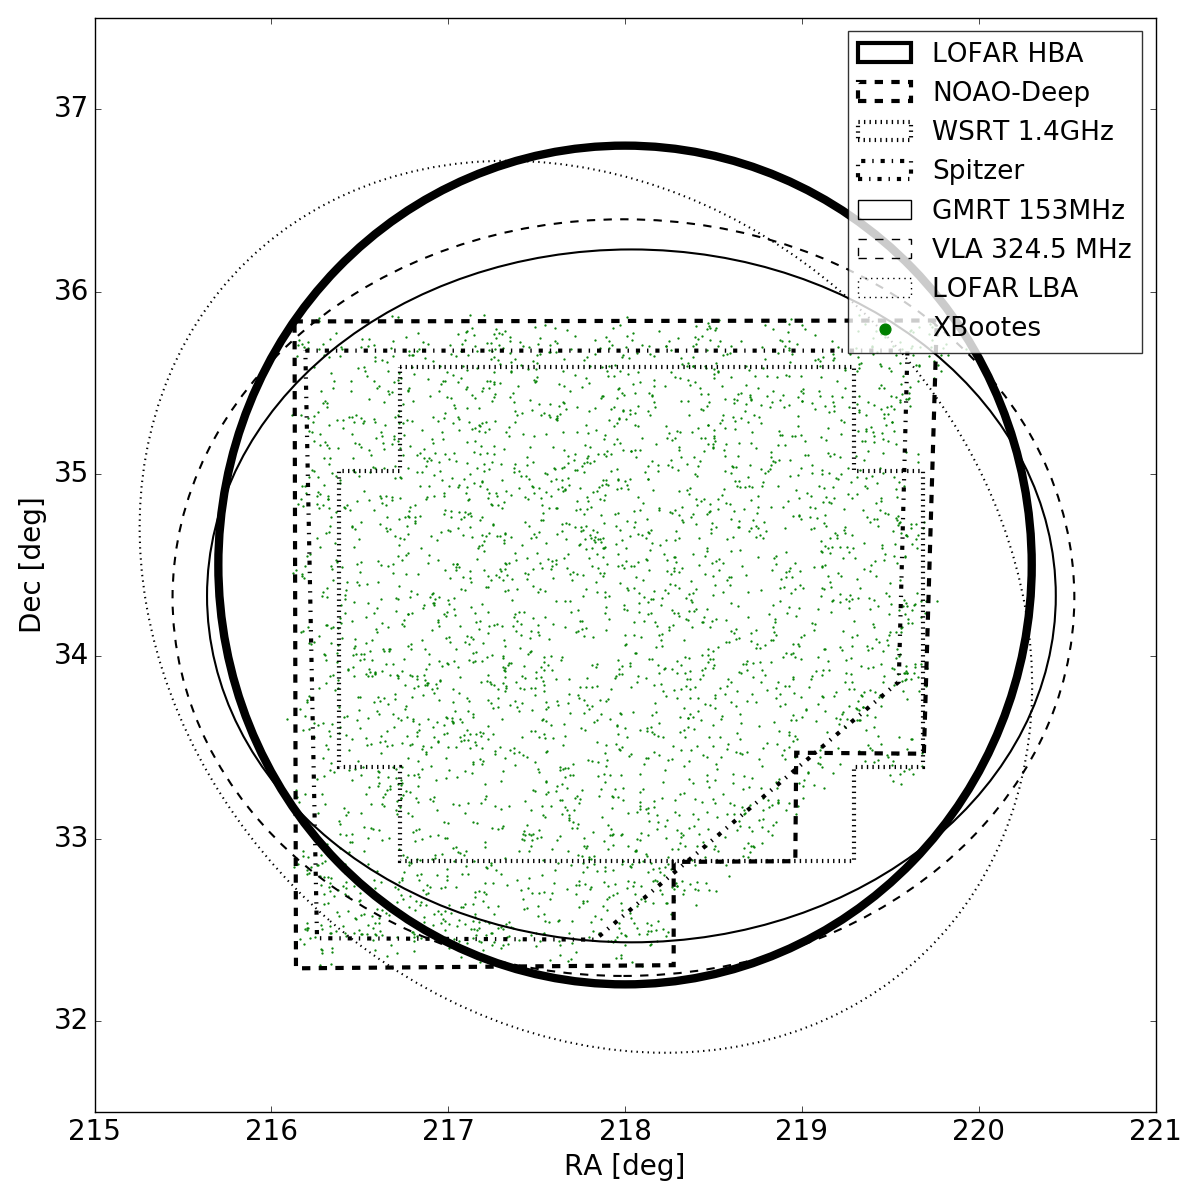
\includegraphics[width=\linewidth]{images/SkyCoverageMap}
\caption{Sky coverage over the Boötes extragalactic field}
\label{bootes-coverage-image}
\end{figure}

It has notably been the subject of very deep Hubble Space Telescope observations, the resolution of which VLBI with LOFAR international can now begin to match.

%
%talk about the field: location, size, history
%
%talk about multi-lambda coverage: put coverage figure here!
%
%\subsection{High-resolution imaging: calibrating the International Baselines}